\documentclass{article}

\usepackage[most]{tcolorbox}
\usepackage{physics}
\usepackage{graphicx}
\usepackage{float}
\usepackage{amsmath}
\usepackage{amssymb}


\usepackage[utf8]{inputenc}
\usepackage[a4paper, margin=1in]{geometry} % Controla los márgenes
\usepackage{titling}

\title{Clase 1 }
\author{Manuel Garcia.}
\date{\today}

\renewcommand{\maketitlehooka}{%
  \centering
  \vspace*{0.05cm} % Espacio vertical antes del título
}

\renewcommand{\maketitlehookd}{%
  \vspace*{2cm} % Espacio vertical después de la fecha
}

\newcommand{\caja}[3]{%
  \begin{tcolorbox}[colback=#1!5!white,colframe=#1!25!black,title=#2]
    #3
  \end{tcolorbox}%
}

\begin{document}
\maketitle

\section{Introduccion }
\subsection{Unidad minia del E-T }
\begin{figure}[H]
  \begin{center}
    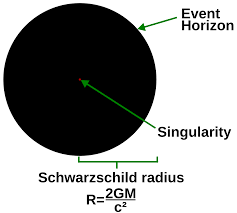
\includegraphics[width=0.4\textwidth]{radio_swa.png}
  \end{center}
\end{figure}
\begin{gather*}
  R = \frac{2MG }{c^2} 
\end{gather*}

Esta es una vision clasica, cuando una estrella muere toda la informacion de la estrella que colapsó en parte se disipa en forma de ondas gravitacionales y otra parte se queda atrapada dentro del radio de schwarzschild. Esto es una paradoja ya que la informacion se pierde. El objetivo de la gravedad cuantica es estudiar que sucede dentro de esta frontera. Esta frontera con su singularidad lo vamos a tratar como una unidad del espacio (o un quantum si queremos verlo así).

\textbf{Ecuacion de campo de Einstein}
\begin{gather*}
  \underset{\text{Tensor de Einstein}}{G _{\mu\nu}} = \textit{cte } \underset{\text{Tensor Metrico de energia}}{T _{\mu\nu}  }
\end{gather*}

De forma cuantizada la podemos escribir como (Teoria Cuantica de Campos Sobre Variedades Curvas): 
\begin{gather*}
  G _{\mu\nu}  = \textit{cte } < T _{\mu\nu}  > \qquad \text{T.C.C.S.V.C} 
\end{gather*}
En esta forma cuantizada Hawking descubrió que la constante es temperatura $ T = \displaystyle\frac{1 }{8\pi M} $. Recordemos que las constantes fundamentales están normalizadas $ \hbar = G=C=\kappa_B=2  $. Notemos que al escribir el radio de schwarzschild $ R=2M  $ se nos va a confundir las distancias con la masa. Además podemos notar que un agujero negro muy masivo tiene una temperatura muy fria, tiende a 0.

\hfill

Calculemos el area de la esfera, Recordemos que podemos enviar masa hacia dentro pero no podemos sacarla ya que violaria la velocidad e la luz. Podemos enviar diferenciales de masa hacia adentro ($ dm  $). Como el radio depende de la masa cuando enviamos $ dm  $ dentro del radio su area tambien aumenta. 
\begin{gather*}
  A = 4\pi R^2 \qquad \rightarrow \qquad A = 4\pi(2M)^2 = 16 \pi M^2 \\
  dA = 8\pi R dR \qquad \rightarrow \qquad dA = 32\pi M dM
\end{gather*}
Entonces el diferencial de masa: $\qquad  dm = \displaystyle\frac{dA }{32 \pi M } $.

\begin{align*}
  dm &= \displaystyle\frac{1 }{8\pi M } \displaystyle\frac{dA }{4 }\\
  dm &= T \underset{\text{Entropia }}{ds } \qquad \text{Esta es la primera ley de la termonidamica}
\end{align*}
Según la segunda ley de la termonidamica $ ds \geq 0  $, por lo tanto  $ dA \geq 0  $. El area se comporta como la entropia. Se puede pensar en los agujeros negros como objetos termicos.

\textbf{Entropia Bekenstein-Hawking } $ S _{BH }  $:
\begin{gather*}
  S _{BH } = \displaystyle\frac{1 }{4 } A  
\end{gather*}
Hoy dia no se conoce exactamente qué nos quiere decir esta expresion. Una de las preguntas que nos hacemos de esta ecuacion es cuales son los grados de libertad microscopicos de $ S _{HB }  $. Una de las teorias que intenta responder esta pregunta es el \textit{Entanglement entropy of black holes}.


\end{document}
